\subsection{RENEW ROI CRITERIA}
%Diagrama2
Region of Interesting is an important element of algorithm because this decides what will be found at image. The mean question in this case is 
the best moment to change ROI. When the comparison of images reaches the threshold 0.925, then ROI is changed. The threshold adopted is 0.8 to 
match case\cite{Eugene}.


\begin{figure}[H]
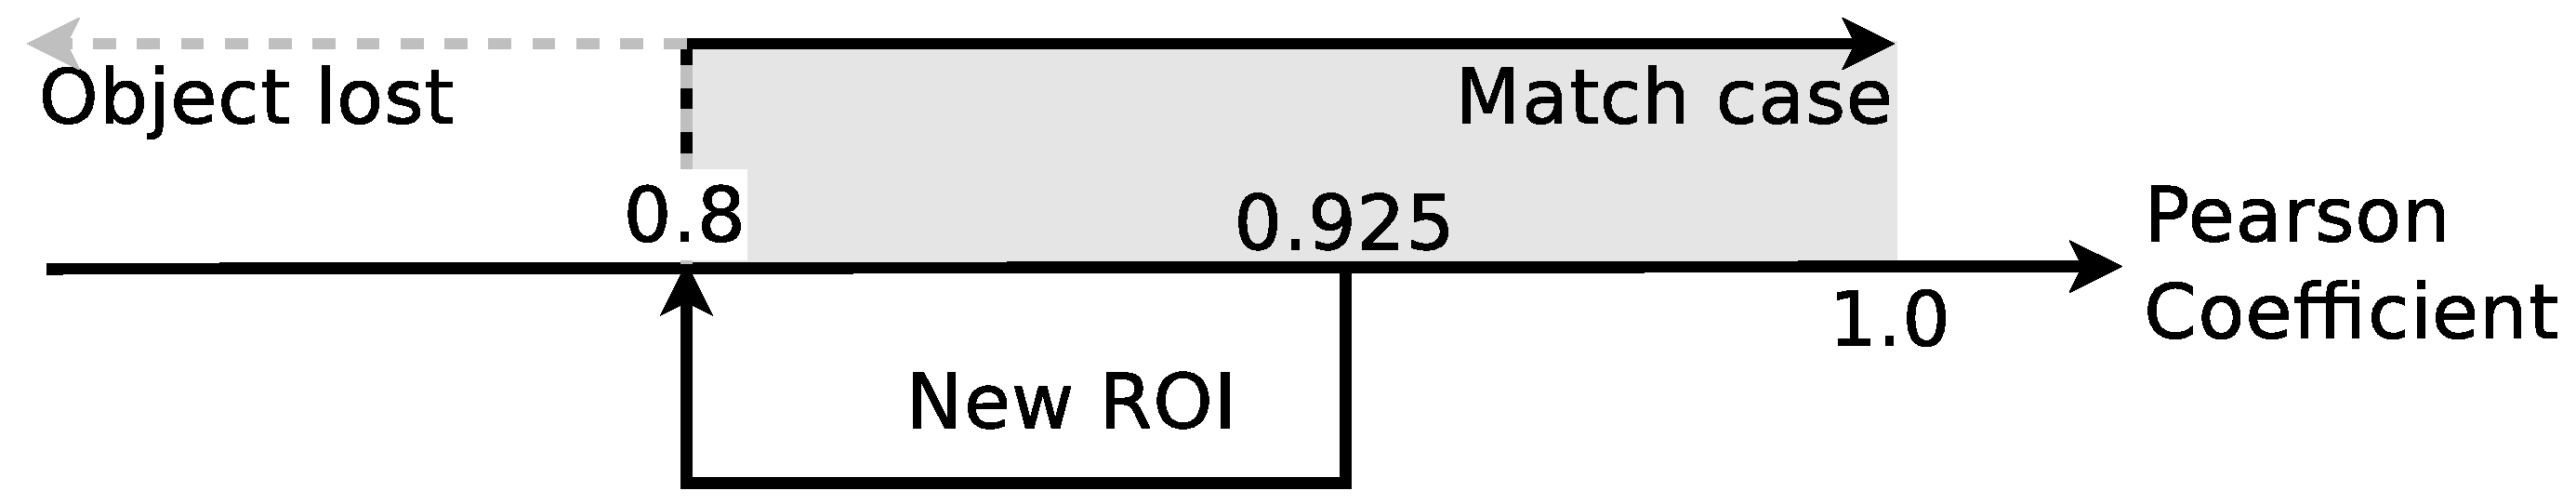
\includegraphics[width=\columnwidth]{images/figure3.eps}
\caption{When the comparison is more than 0.8, including numbers bigger than 0.925, the target was matched. But if two images are compared 
and PCC is less than 0.925, so the ROI changes to the last ROI compared.}
\end{figure}

The system needs to have high level of reliability, so the threshold adopted contributes to an operation with minimum of mistakes.
